\documentclass[]{article}

\usepackage{amsmath}
\usepackage{amssymb}
\usepackage{graphicx}
\usepackage[utf8]{inputenc} 
\usepackage{subcaption}
\usepackage{caption}
\usepackage{hyperref} 
%opening
\title{}
\author{}

\begin{document}

\maketitle

\begin{abstract}
\end{abstract}


\section{Weighted operator tests}
\begin{figure}
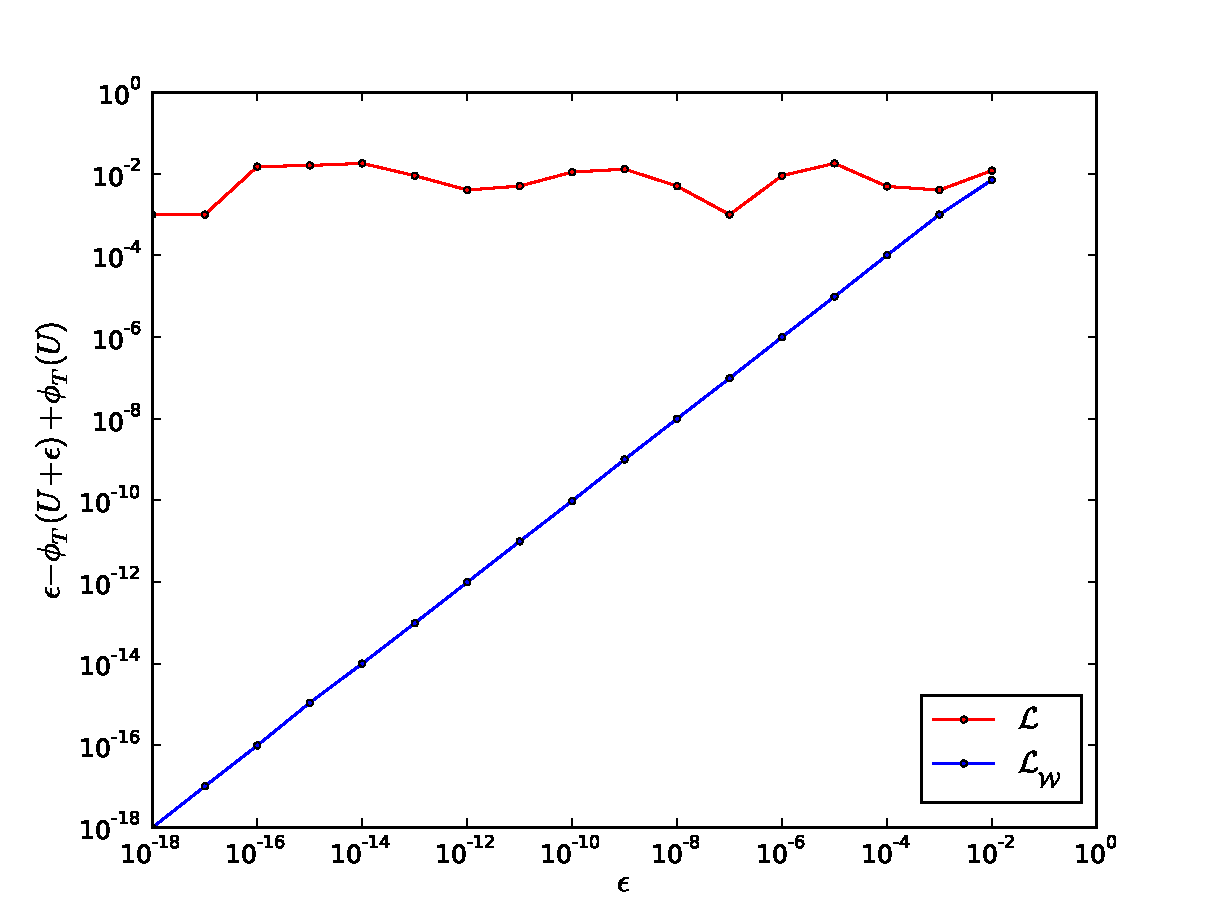
\includegraphics[width=0.9\textwidth]{epsilon_dependence_M1000_N40_1dim.pdf}
\caption{For the red plot, the coarse time-stepper was calculated without weights and for two independent function evaluations. For the blue plot we used weighted operators calculated with the same realizations, microscopic parameters and random time paths. For both simulations we used $N=40$, $M=1000$ and a time horizon of 5 steps in the coarse time steppers. We only collected statistics of one particle.}
\label{fig:epsilon}
\end{figure}

\end{document}
